%!TEX root = main.tex

Considere una fuente $\mathcal{F}$ con una distribución  de probabilidad $\mathcal{P}=\{0\text{.}20,0\text{.}15,0\text{.}15,0\text{.}10,0\text{.}10,0\text{.}30\}$ construya un código con longitud promedio de palabra $L$, tal que
$$H(\mathcal{F})\leq L \leq H(\mathcal{F})+1.$$
\begin{sols}
 Primero la entropía que calcularemos es en base $2,$ por lo que codificaremos en un alfabeto binario. Por la distribución de probabilidad sabemos que la entropía viene dada por  
 \begin{align*}
  H(\mathcal{F})&=0.20\log_2(0.20)+0.15\log_2(0.15)+0.15\log_2(0.15)+0.10\log_2(0.10)\\
  &\phantom{++}+0.10\log_2(0.10)+0.30\log_2(0.30)\\
  &\approx 2.47095.
  \end{align*} 
  Por lo que estamos buscando un código con longitud promedio de palabra $L$ tal que
  $$2.47095\leq L\leq 3.47095.$$
  Sabemos por una proposición vista que siempre existe un código unívocamente decodificable con una longitud promedio $L$ que cumpla la desigualdad previa. Tenemos múltiples formas de hacerlo por lo que se presentaran dos códigos que cumplen.\\

  Primero en la demostración de la proposición se toman longitudes de palabra
  $$l_i=\left\lceil\log_2\dfrac{1}{p_i}\right\rceil$$
  De esta manera nuestras longitudes de palabra son
  \begin{align*}
        l_1&=\left\lceil\log_2\dfrac{1}{0.20}\right\rceil=3,\\
        l_2&=\left\lceil\log_2\dfrac{1}{0.15}\right\rceil=3,\\
        l_3&=\left\lceil\log_2\dfrac{1}{0.15}\right\rceil=3,\\
        l_4&=\left\lceil\log_2\dfrac{1}{0.10}\right\rceil=4,\\
        l_5&=\left\lceil\log_2\dfrac{1}{0.10}\right\rceil=4,\\
        l_6&=\left\lceil\log_2\dfrac{1}{0.30}\right\rceil=2.\\
  \end{align*}
  Note que la longitud promedio de palabra para un código con esas longitudes seria
  \begin{align*}
      L&=(0.20+0.15+0.15)3+(0.10+0.10)4+0.30\cdot 2\\
      &=2.9
  \end{align*}
  que cumple la desigualdad. Primero realizamos un árbol de altura 2
  \begin{center}
       \begin{tikzpicture}[level 1/.style={sibling distance=25mm}, level 2/.style={sibling distance=15mm}]

            \node[hollow](0){}
            child{node[solid]{}
                child{node[green node]{}}
                child{node[red node]{}}}  
            child{node[solid]{}
                child{node[red node]{}}
                child{node[red node]{}}}
;
\end{tikzpicture}
    \end{center}
    Luego el de altura 3
    \begin{center}
       \begin{tikzpicture}[level 1/.style={sibling distance=25mm}, level 2/.style={sibling distance=20mm}, level 3/.style={sibling distance=15mm}]
            \node[hollow](0){}
            child{node[solid]{}
                child{node[green node]{}}
                child{node[red node]{}}}  
            child{node[solid]{}
                child{node[solid]{}
                    child{node[green node]{}}
                    child{node[green node]{}}}
                child{node[solid]{}
                    child{node[green node]{}}
                    child{node[red node]{}}}}
;
            
\end{tikzpicture}
    \end{center}
    Por último el de altura 4
    \begin{center}
       \begin{tikzpicture}[level 1/.style={sibling distance=25mm}, level 2/.style={sibling distance=20mm}, level 3/.style={sibling distance=15mm}]
            \node[hollow](0){}
            child{node[solid]{}
                child{node[green node]{}}
                child{node[box node]{}}}  
            child{node[solid]{}
                child{node[solid]{}
                    child{node[green node]{}}
                    child{node[green node]{}}}
                child{node[solid]{}
                    child{node[green node]{}}
                    child{node[solid]{}
                        child{node[green node]{}}
                        child{node[green node]{}}}}}
;
            
\end{tikzpicture}
    \end{center}
Si asignamos ceros a las ramas de la izquierda y unos a las de la derecha obtenemos el siguiente código
\begin{center}
  \begin{tabular}{|c|c|c|c|c|c|}
  \hline
$0.20$ & $0.15$ & $0.15$ & $0.10$ & $0.10$ & $0.30$\\
\hline
$100$ & $101$ & $110$ & $1110$ & $1111$ & $00$\\
\hline
 \end{tabular}
 \end{center}
 Donde a cada probabilidad de la d.p. le asignamos un respectivo código de la longitud establecida.\\

 La otra posibilidad para un código que cumpla la desigualdad, es encontrar un código de longitud promedio de palabra constante. Ya que note que si hacemos $L=3$, también cumplimos la desigualdad, para eso, sigamos el algoritmo de Tunstall. Consideramos $D_z=2$ y $D_u=6.$ Seguiremos por pasos el algoritmo:

\textbf{Paso 1:}
\begin{itemize}
    \item[a)] Queremos un $n$, tal que $2^n\geq 6$, por lo que escogeremos $n=3$, ya que es el primer natural que cumple la desigualdad, esta será nuestra longitud de palabra.
    \item[b)] Tenemos que $k=\left\lfloor\dfrac{2^3-1}{6-1}\right\rfloor=\left\lfloor\dfrac{7}{5}\right\rfloor=1.$ Dado que este es el número de nodos internos, podemos inferir en este paso que sólo tendremos a la raíz como nodo interno.
    \item[c)] Por lo anterior, tenemos que $M=1+1(6-1)=6.$ Es decir que el número de mensajes a codificar es el mismo que el de símbolos de la fuente.
\end{itemize}
\textbf{Paso 2:}
 Note que en este paso del algoritmo como resaltamos antes solo asignamos hijos a la raíz, cuando hacemos $j=1$, ya que $k=1.$ Por  lo que el árbol construido es el siguiente:
 \begin{center}
       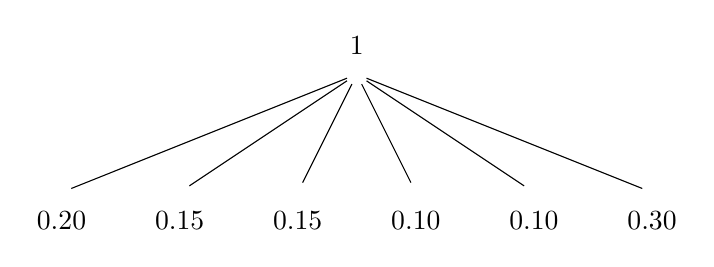
\begin{tikzpicture}

            \node[solid, label=above:{1}](0){}
                child{node[solid, label=below:{$0.20$}]{}}
                child{node[solid, label=below:{$0.15$}]{}}
                child{node[solid, label=below:{$0.15$}]{}}
                child{node[solid, label=below:{$0.10$}]{}}
                child{node[solid, label=below:{$0.10$}]{}}
                child{node[solid, label=below:{$0.30$}]{}}
;
\end{tikzpicture}
    \end{center}
De esta manera el código de longitud promedio constante 3 es
\begin{center}
  \begin{tabular}{|c|c|c|c|c|c|}
  \hline
$0.20$ & $0.15$ & $0.15$ & $0.10$ & $0.10$ & $0.30$\\
\hline
$000$ & $001$ & $010$ & $011$ & $100$ & $101$\\
\hline
 \end{tabular}
 \end{center}

\end{sols}